\section{Survival detail}
\label{app:survival}

\subsection*{Segment summary under the primary event definition}

\begin{longtable}[]{@{}lrrrrr@{}}
\toprule\noalign{}
Segment & Episodes & Events & Event rate & $S(12)$ & $S(24)$ \\
\midrule\noalign{}
\endhead
CPV-32 & 1,152 & 152 & 0.1319 & 0.9583 & 0.9400 \\
CPV-35 & 564 & 115 & 0.2039 & 0.9357 & 0.9043 \\
CPV-48 & 790 & 92 & 0.1165 & 0.9609 & 0.9323 \\
CPV-72 & 1,294 & 185 & 0.1430 & 0.9533 & 0.9391 \\
\bottomrule\noalign{}
\end{longtable}

Multivariate log-rank across the four segments: statistic 23.45, $p = 3.26 \times 10^{-5}$.

\subsection*{Cox model, full output}

\begin{longtable}[]{@{}>{\raggedright\arraybackslash}p{4.6cm}rrrr@{}}
\toprule\noalign{}
Covariate & $\hat\beta$ & HR & 95\,\% CI & $p$ \\
\midrule\noalign{}
\endhead
Framework agreement & 0.5600 & 1.751 & [1.435, 2.136] & $3.38\times 10^{-8}$ \\
Validated SIREN & 0.0787 & 1.082 & [0.885, 1.323] & 0.443 \\
Award year (centred) & 0.1016 & 1.107 & [1.066, 1.149] & $1.21\times 10^{-7}$ \\
CPV-35 (ref. CPV-32) & 0.4405 & 1.553 & [1.218, 1.981] & $3.83\times 10^{-4}$ \\
CPV-48 & $-0.1892$ & 0.828 & [0.638, 1.073] & 0.153 \\
CPV-72 & 0.0540 & 1.056 & [0.850, 1.310] & 0.624 \\
Normandie (ref. Bretagne) & $-0.2230$ & 0.800 & [0.640, 1.000] & 0.050 \\
Pays de la Loire & 0.0028 & 1.003 & [0.815, 1.234] & 0.979 \\
\bottomrule\noalign{}
\end{longtable}

3,800 awarded procurement episodes, 544 events, 8 covariates, partial AIC 8,537.99, in-sample concordance 0.6257.

\subsection*{Proportional-hazards diagnostics}

\begin{longtable}[]{@{}>{\raggedright\arraybackslash}p{6.5cm}rr@{}}
\toprule\noalign{}
Covariate & Test statistic & $p$ \\
\midrule\noalign{}
\endhead
Award year (centred) & 70.73 & $4.09\times 10^{-17}$ \\
Framework agreement & 7.04 & 0.0080 \\
Validated SIREN & 6.76 & 0.0093 \\
CPV-72 & 3.72 & 0.0537 \\
Pays de la Loire & 2.45 & 0.117 \\
Normandie (ref. Bretagne) & 0.61 & 0.436 \\
CPV-48 & 0.67 & 0.413 \\
CPV-35 (ref. CPV-32) & 0.04 & 0.840 \\
\bottomrule\noalign{}
\end{longtable}

Three covariates reject the constant-effect null. The award-year violation is severe and structurally
expected, because award year is confounded with follow-up length. \emph{The two segment coefficients that
carry the report's comparative claims are the two that pass the diagnostic most comfortably.}

\subsection*{Parametric family comparison}

\begin{longtable}[]{@{}lrrrr@{}}
\toprule\noalign{}
Family & Parameters & Log-likelihood & AIC & BIC \\
\midrule\noalign{}
\endhead
Generalised gamma & 3 & $-3{,}757.49$ & \textbf{7,520.99} & \textbf{7,539.72} \\
Log-normal & 2 & $-3{,}784.62$ & 7,573.24 & 7,585.73 \\
Log-logistic & 2 & $-3{,}807.28$ & 7,618.57 & 7,631.05 \\
Weibull & 2 & $-3{,}814.68$ & 7,633.35 & 7,645.84 \\
Exponential & 1 & $-3{,}829.66$ & 7,661.31 & 7,667.55 \\
\bottomrule\noalign{}
\end{longtable}

\begin{figure}[htbp]
\centering
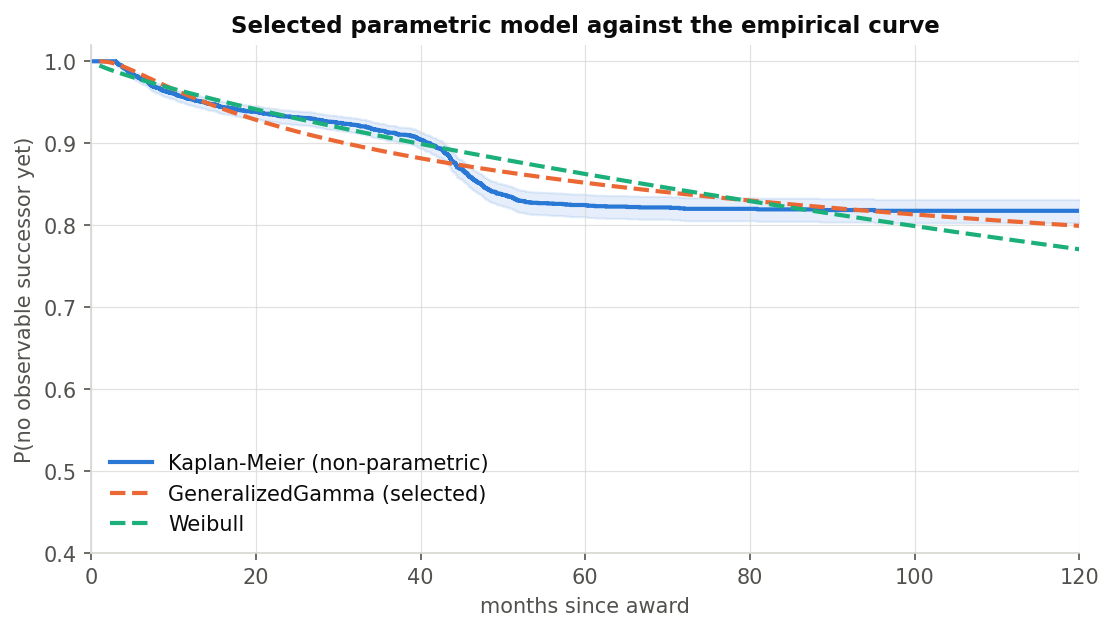
\includegraphics[width=0.8\linewidth]{figures/appD_parametric_vs_empirical.png}
\caption{Fitted parametric survival functions against the empirical Kaplan--Meier curve. Every smooth family
flattens the observed 36--48 month re-procurement shoulder, which is precisely the feature of operational interest. This is
why the reported 12- and 24-month probabilities are read off the empirical estimator, even though the
generalised gamma has the lowest AIC and BIC.}
\label{fig:appd-param}
\end{figure}

\subsection*{Sensitivity arms}

\begin{longtable}[]{@{}>{\raggedright\arraybackslash}p{3.4cm}rrrrr@{}}
\toprule\noalign{}
Arm & Events & Rate & $P(\le 12\text{m})$ & $P(\le 24\text{m})$ & Median observed gap \\
\midrule\noalign{}
\endhead
\texttt{M\_B @ 0.80} strict & 296 & 0.0779 & 2.37\,\% & 3.23\,\% & 35.7 m \\
\texttt{M\_B @ 0.70} primary & 544 & 0.1432 & 4.62\,\% & 6.73\,\% & 31.8 m \\
\texttt{M\_B @ 0.60} loose & 853 & 0.2245 & 8.00\,\% & 11.47\,\% & 26.6 m \\
\texttt{M\_C @ 0.70} contrast & 1,332 & 0.3505 & 12.21\,\% & 17.98\,\% & 26.1 m \\
\bottomrule\noalign{}
\end{longtable}

\subsection*{Buyer-stratified Cox sensitivity}
Robust score-based inference is one way to address clustered Cox data \citep{linwei1989}; the sensitivity here instead changes the estimand by stratifying on buyer and estimating effects only from within-buyer comparisons.

The primary within-buyer model contains 2,188 episodes, 511 events and 195 buyers. Each buyer receives its own
baseline hazard, so fixed buyer characteristics are absorbed. Candidate-pool size is not: it varies within 473
of the 514 buyers carrying multiple cohort episodes.

\begin{longtable}[]{@{}>{\raggedright\arraybackslash}p{5.2cm}rrr@{}}
\toprule\noalign{}
Covariate & HR & 95\,\% CI & $p$ \\
\midrule\noalign{}
\endhead
Framework agreement & 1.497 & [1.150, 1.948] & 0.0027 \\
Award year (centred) & 1.015 & [0.967, 1.065] & 0.547 \\
CPV-35 (ref. CPV-32) & 1.213 & [0.866, 1.699] & 0.262 \\
CPV-48 & 0.482 & [0.346, 0.672] & $1.7\times10^{-5}$ \\
CPV-72 & 0.831 & [0.627, 1.100] & 0.196 \\
\bottomrule\noalign{}
\end{longtable}

Across the four linkage arms, the CPV-35 estimates are 1.265, 1.213, 1.280 and 1.109; the CPV-48 estimates
are 0.477, 0.482, 0.589 and 0.744; and the framework estimates are 1.128, 1.497, 1.664 and 1.459. Directional
stability is distinct from significance in every arm: the strict framework estimate is imprecise.

\begingroup
\setlength{\tabcolsep}{4.5pt}
\begin{longtable}[]{@{}>{\raggedright\arraybackslash}p{5.4cm}rrrrr@{}}
\toprule\noalign{}
Robustness check & Episodes & Events & $P(\le 12\text{m})$ & CPV-35 HR & Framework HR \\
\midrule\noalign{}
\endhead
Main & 3,800 & 544 & 4.62\,\% & 1.553 & 1.751 \\
Excluding the borderline band $[0.65,0.75]$ & 3,520 & 411 & 3.72\,\% & 1.780 & 1.616 \\
Re-censoring template-risk links & 3,800 & 371 & 2.64\,\% & 1.541 & 1.692 \\
\bottomrule\noalign{}
\end{longtable}
\endgroup

The borderline band removes 280 episodes, of which 133 are events and 147 censored. The template-risk check
re-censors 173 of the 544 accepted links (31.8\,\%): 65 carry word-level similarity below 0.50, and 127 share
their successor episode with another anchor.

\subsection*{Detectability diagnostic}

\begin{longtable}[]{@{}>{\raggedright\arraybackslash}p{5.6cm}rrr@{}}
\toprule\noalign{}
Variable & Linked mean & Censored mean & SMD \\
\midrule\noalign{}
\endhead
log(candidate pool size) & 4.787 & 3.972 & $+0.470$ \\
Candidate pool size & 274.3 & 188.6 & $+0.285$ \\
Episode text length & 1,611 & 1,087 & $+0.262$ \\
Framework agreement & 0.2647 & 0.1867 & $+0.187$ \\
Administrative follow-up (months) & 70.65 & 65.38 & $+0.146$ \\
Award year & 2020 & 2020 & $-0.137$ \\
Validated SIREN & 0.3107 & 0.3409 & $-0.065$ \\
Notices per episode & 1.978 & 2.045 & $-0.058$ \\
Reliable duration present & 0.2445 & 0.2518 & $-0.017$ \\
\bottomrule\noalign{}
\end{longtable}

Sensitivity model adding $\log(1 + \text{pool size})$ to the main specification:

\begin{longtable}[]{@{}>{\raggedright\arraybackslash}p{5.0cm}rrr@{}}
\toprule\noalign{}
Covariate & HR, main & HR, adjusted & $p$, adjusted \\
\midrule\noalign{}
\endhead
Framework agreement & 1.751 & 1.617 & $2.6\times 10^{-6}$ \\
Validated SIREN & 1.082 & 0.983 & 0.87 \\
Award year (centred) & 1.107 & 1.145 & $4.1\times 10^{-11}$ \\
CPV-35 (ref. CPV-32) & 1.553 & 1.512 & $8.5\times 10^{-4}$ \\
CPV-48 & 0.828 & 0.769 & 0.048 \\
CPV-72 & 1.056 & 0.977 & 0.83 \\
Normandie (ref. Bretagne) & 0.800 & 0.796 & 0.046 \\
Pays de la Loire & 1.003 & 0.975 & 0.81 \\
log(candidate pool size) & --- & 1.184 & $6.0\times 10^{-9}$ \\
\bottomrule\noalign{}
\end{longtable}

\subsection*{Segment-stratified watch list}

The one operational artifact derived from these curves is a segment-stratified list: for each of the four CPV
segments, the five still-unlinked episodes awarded in 2021 or later with the highest conditional probability
of showing a successor within twelve months. It is read off the segment-stratified Kaplan--Meier curves, not
off the Cox model, and it is stratified deliberately. Because the conditional probability is a function of
segment and age alone, an unstratified ranking would simply return the highest-hazard segment at the age
closest to the shoulder, implying an individual-level precision that the out-of-time concordance of 0.479
does not support. The file is
\texttt{data/processed/boamp/segment\_watch\_km.csv}.
